\documentclass{beamer}
\usepackage{fontspec}
\usepackage{subfig}
\usepackage{unicode-math}
\usepackage{tabularray}
\usepackage{ragged2e}
\usepackage{array}
\usepackage{setspace}

\usetheme{metropolis}
\setbeamertemplate{footline}{}
\usefonttheme{professionalfonts}
\usefonttheme{serif}
\setmainfont{DejaVu Sans}
\setmathfont{XITS Math}

\title{Անտենաների թերությունների և ճառագայթվող էլեկտրամագնիսական դաշտի հետազոտումը ջերմաառաձգական օպտիկական ինդիկատորով մանրադիտակի օգնությամբ}
\author{Ուսանող՝ Սիմոնյանց Դավիթ}
\date{}
\institute{ԵՐԵՎԱՆԻ ՊԵՏԱԿԱՆ ՀԱՄԱԼՍԱՐԱՆ / ՖԻԶԻԿԱՅԻ ԻՆՍՏԻՏՈՒՏ}

\newcommand{\sectslides}{0}
\newcounter{currslide}
\newcommand{\resetCountingSlides}[1]{
    \renewcommand{\sectslides}{#1}
    \setcounter{currslide}{1}
}
\newcommand{\countSlide}{\addtocounter{currslide}{1}}
\newcommand{\showSlide}{\thecurrslide/\sectslides}
\newcommand{\showCountSlide}{\showSlide \countSlide}
\newcommand{\frametitlecounted}[1]{\frametitle{#1 \hfill \fontsize{10}{10} \selectfont \showCountSlide}}

\begin{document}
\hyphenpenalty=10000
\exhyphenpenalty=10000

\begin{frame}
\titlepage
\end{frame}

\resetCountingSlides{3}

\begin{frame}
\frametitlecounted{Ներածություն}

Անտենաները կարևոր դեր են խաղում հեռահաղորդակցման ոլորտում, հնարավորություն տալով հաղորդել և ընդունել էլեկտրամագնիսական ալիքներ։

\begin{figure}[ht]
  \centering
  \begin{minipage}[b]{0.45\linewidth}
    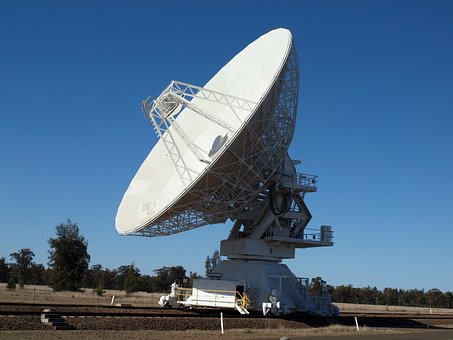
\includegraphics[width=\linewidth]{data/presentation/antenna-1.jpg}
  \end{minipage}
  \hfill
  \begin{minipage}[b]{0.45\linewidth}
    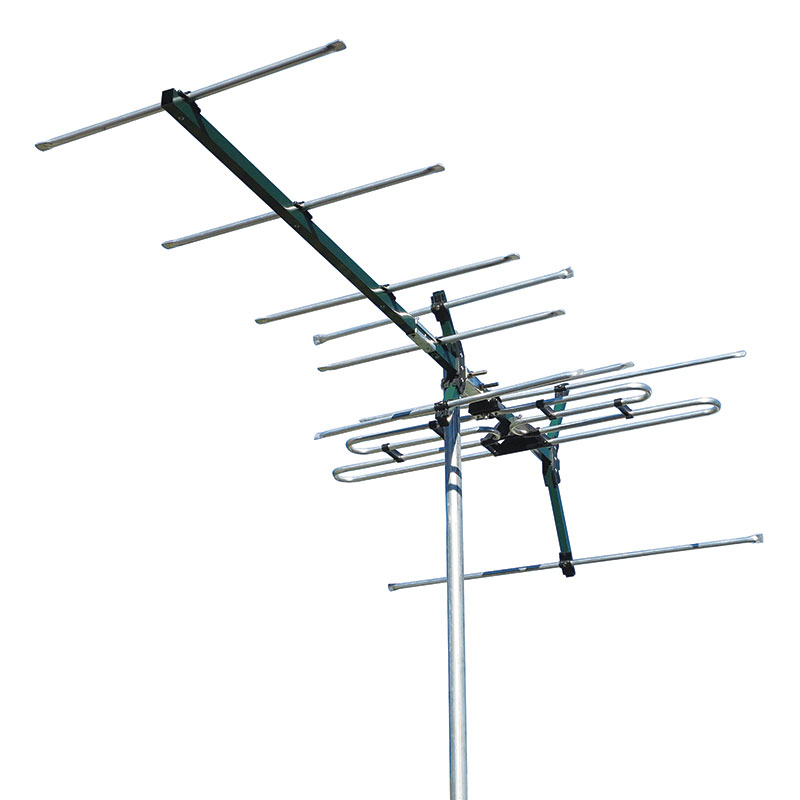
\includegraphics[width=\linewidth]{data/presentation/antenna-2.jpg}
  \end{minipage}
\end{figure}

\end{frame}


\begin{frame}
\frametitlecounted{Ներածություն}

Անտենաներում հայտնվող թերությունները բերում են անցանկալի խնդիրների, օրինակ՝
\begin{itemize}
    \item Ազդանշանների թուլացումներ կամ կորուստներ
    \item Ավելցուկային անցանկալի ինտերֆերենցիաներ
    \item Հաճախային շեղումներ
    \item Ազդանշանների աղավաղումներ
\end{itemize}
Ընդհանուր դեպքում՝ թերությունները ազդեցություն են թողնում անտենայից ճառագայթվող էլեկտրամագնիսական դաշտի վրա։

\end{frame}

\begin{frame}
\frametitlecounted{Ներածություն}

Էլեկտրամագնիսական դաշտը հետազոտելու միջոցներ՝

\begin{itemize}
    \item Սկանավորման տեխնիկա՝
        \begin{itemize}
            \item Սկանավորող ջերմային մանրադիտակ (Scanning thermal microscope (SThm))
            \item Մերձադաշտի սկանավորման օպտիկական մանրադիտակ (Near-field scanning optical microscope (NSOM))
        \end{itemize}
    \item Ջերմաառաձգական օպտիկական ինդիկատորով մանրադիտակ (ՋԱՕԻՄ)
\end{itemize}

\end{frame}

\resetCountingSlides{4}

\begin{frame}
\frametitlecounted{ՋԱՕԻՄ}
    ՋԱՕԻՄ֊ի սզկբունքային սխեման՝
    \begin{figure}
        \centering
        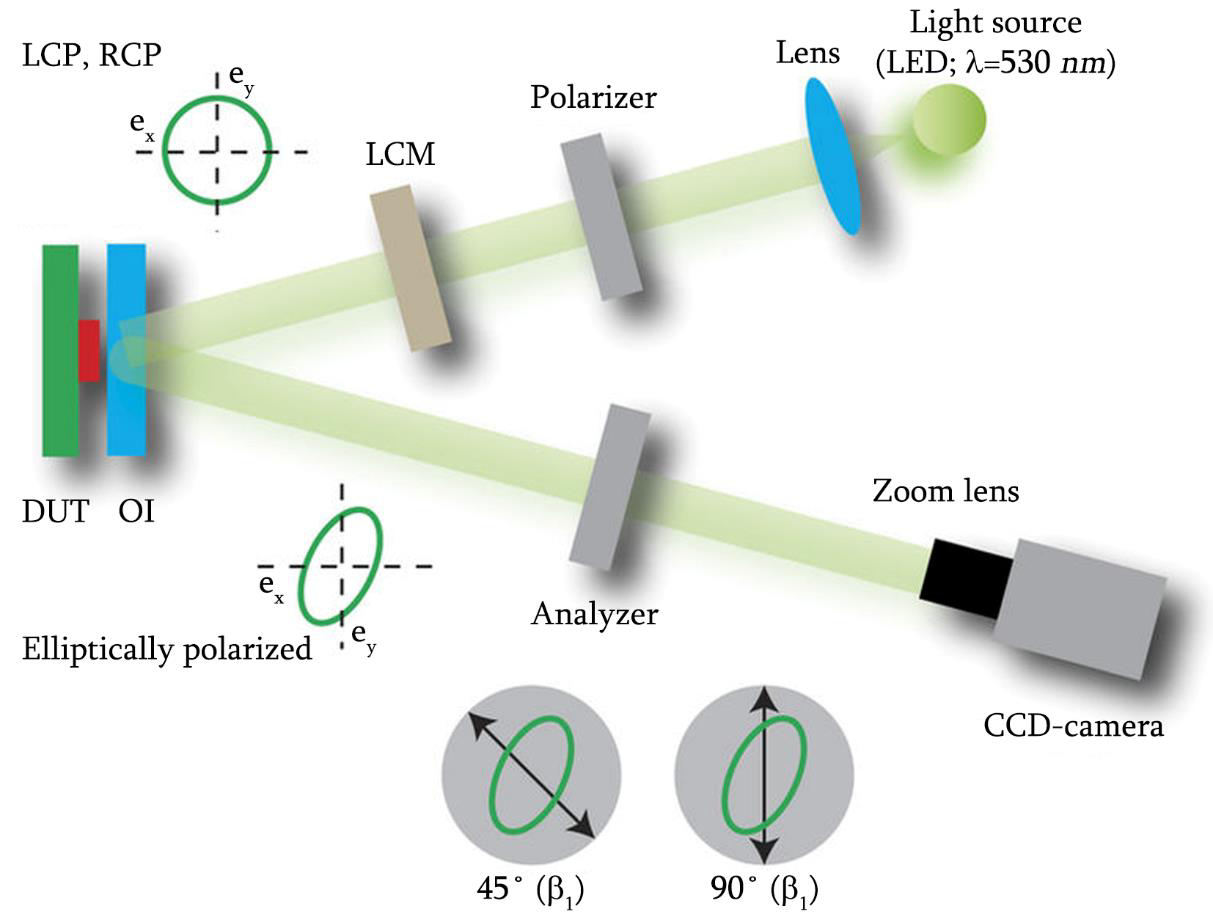
\includegraphics[width=0.9\textwidth]{data/TEOIM/0.jpg}
    \end{figure}
\end{frame}

\begin{frame}
\frametitlecounted{ՋԱՕԻՄ}
    Ֆոտոէլաստիկ երևույթը օպտիկական ինդիկատորում՝
    \begin{figure}
        \centering
        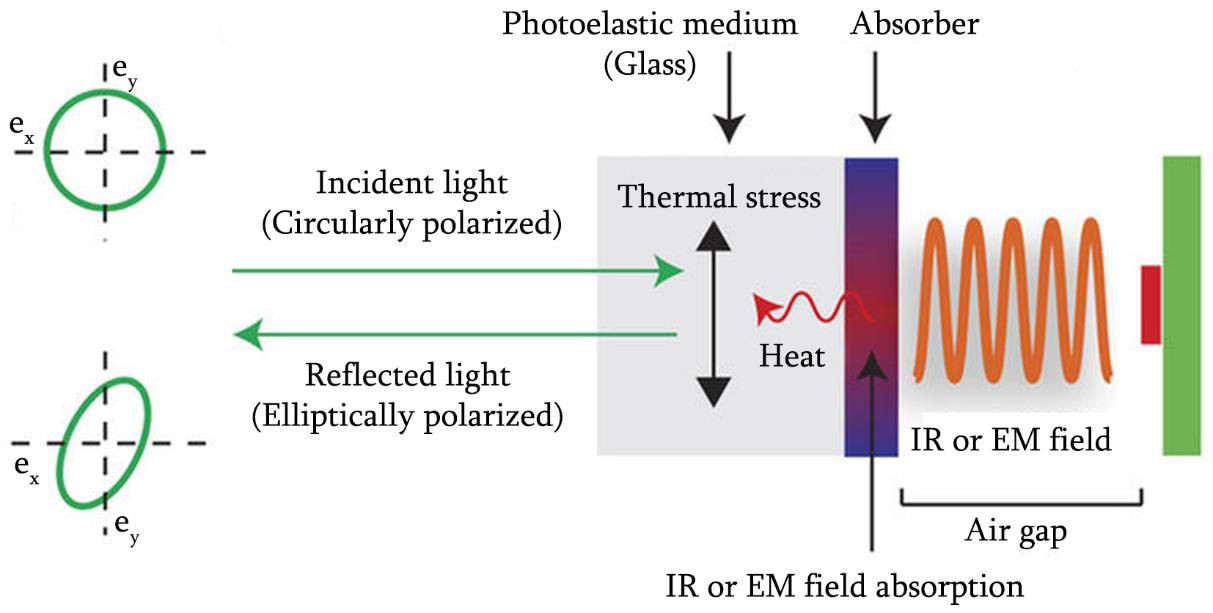
\includegraphics[width=\textwidth]{data/TEOIM/1.jpg}
    \end{figure}
\end{frame}

\begin{frame}
\frametitlecounted{ՋԱՕԻՄ}
    Կապը $q$ ջերմային բաշխվածության և $\beta_1$, $\beta_2$ գծային երկբեկման միջև՝
    \begin{flalign*}
    q &= \frac {\lambda}{2\pi dS} \frac{1 - \nu}{\alpha Ek}
    \left( 2 \frac{\partial^2 \beta_2}{\partial x \partial y} +  \frac{\partial^2 \beta_1}{\partial x^2} - \frac{\partial^2\beta_1}{\partial y^2} \right)
    \end{flalign*}
    {\fontsize{10}{10} \selectfont
        որտեղ՝ \\
        $S$֊ը լարման օպտիկական հաստատունն է, \\
        $\lambda$֊ն ընկնող լույսի ալիքի երկարությունն է, \\
        $d$֊ն ինդիկատորի հաստությունն է, \\
        $\alpha$֊ն ջերմային ընդարձակման գործակիցն է, \\
        $\nu$֊ն Պուասոնի գործակիցն է, \\
        $E$֊ն Յունգի մոդուլն է, \\
        $k$֊ն ինդիկատորի էֆեկտիվ ջերմահաղորդականությունն է։
    }
    
\end{frame}

\begin{frame}
\frametitlecounted{ՋԱՕԻՄ}
    {\fontsize{10}{10} \selectfont Էլեկտրամագնիսական դաշտի կորուստները՝ \\
    էլեկտրական դաշտի համար դիէլեկտրիկ միջավայրում՝}
    \begin{flalign*}
    q &= \frac{\omega}{2} \varepsilon'' |E|^2,
    \end{flalign*} \\
    {\fontsize{10}{10} \selectfont մագնիսական դաշտի համար հաղորդիչ միջավայրում՝}
    \begin{flalign*}
        q &= \frac{P_{av}}{V} = \frac{R_s}{2t}|H_t|^2, \\
    \label{eq:TD_vs_Ht}
    P_{av} &= \int\frac{R_s}{2}|H_t|^2dS, \\
    R_s &= \sqrt{\frac{\omega \mu}{2\sigma}} = \frac{1}{\sigma \delta_s},
    \end{flalign*}
    
\end{frame}

\resetCountingSlides{2}

\begin{frame}
\frametitlecounted{Տվյալների հավաքագրումը և վերամշակումը}
{\fontsize{10}{1} \selectfont Տվյալների հավաքագրման քայլերի հերթականությունը՝}
\vspace{-5pt}
\begin{figure}
    \centering
    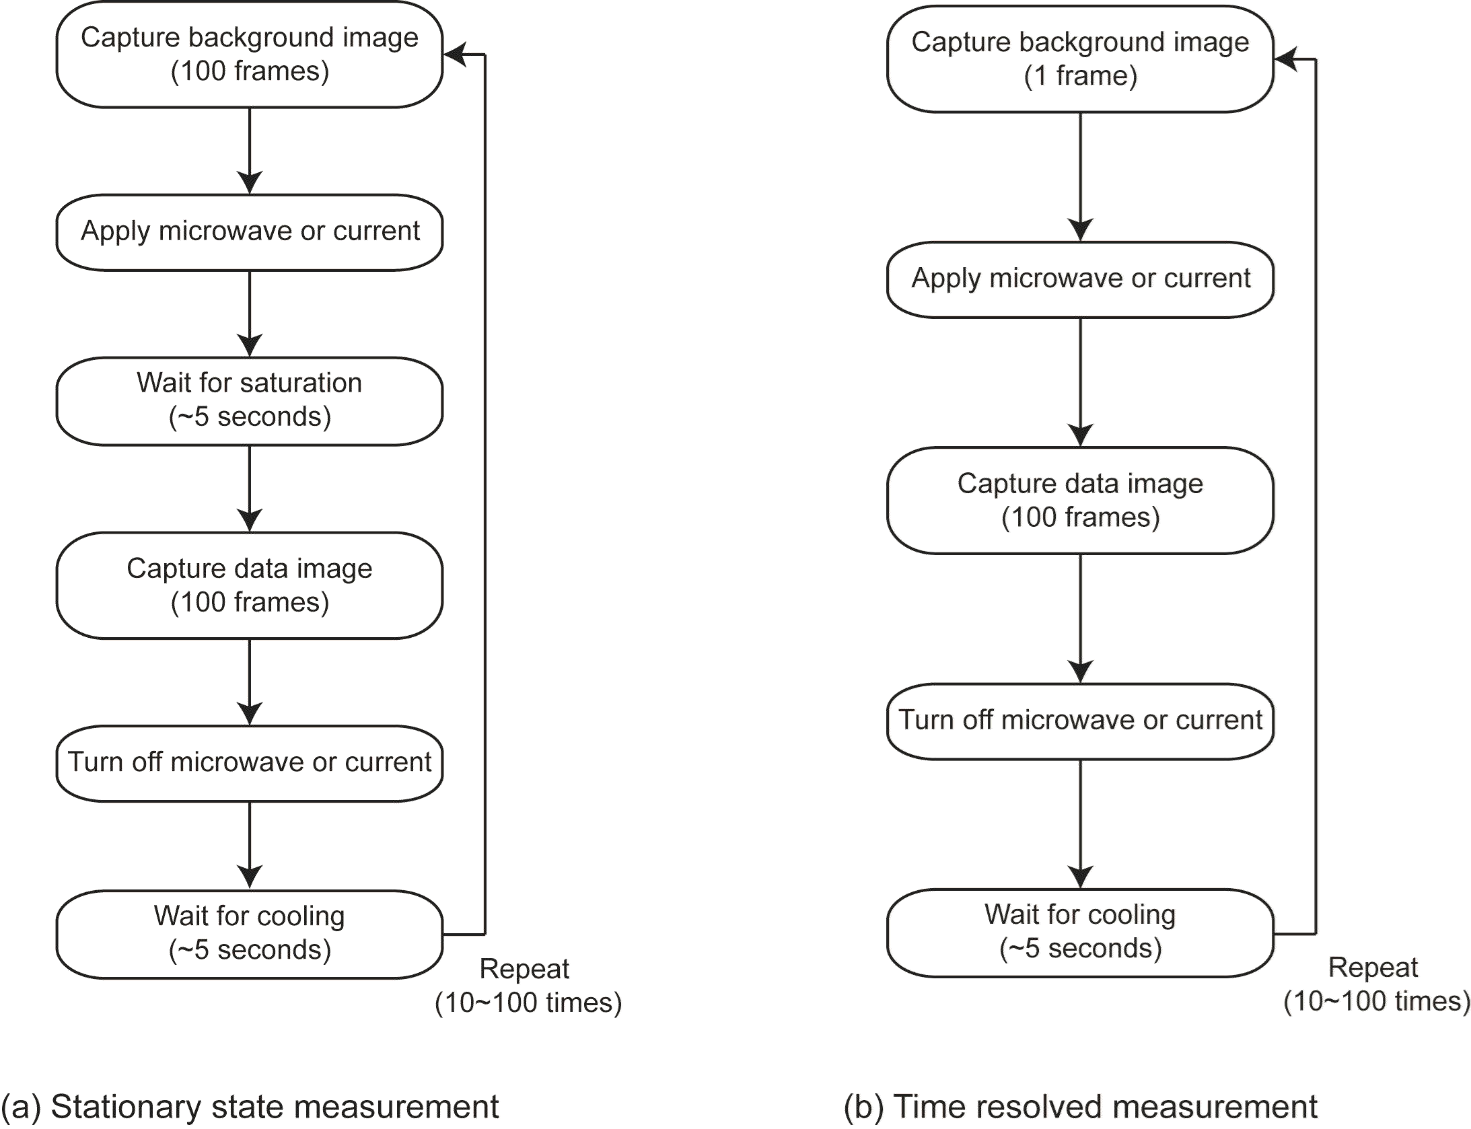
\includegraphics[width=0.9\textwidth]{data/TEOIM/3.png}
\end{figure}
\end{frame}

\begin{frame}
\frametitlecounted{Տվյալների հավաքագրումը և վերամշակումը}
Հարթեցման և դիֆերենցման պրոցեսները՝

\begin{figure}
    \centering
    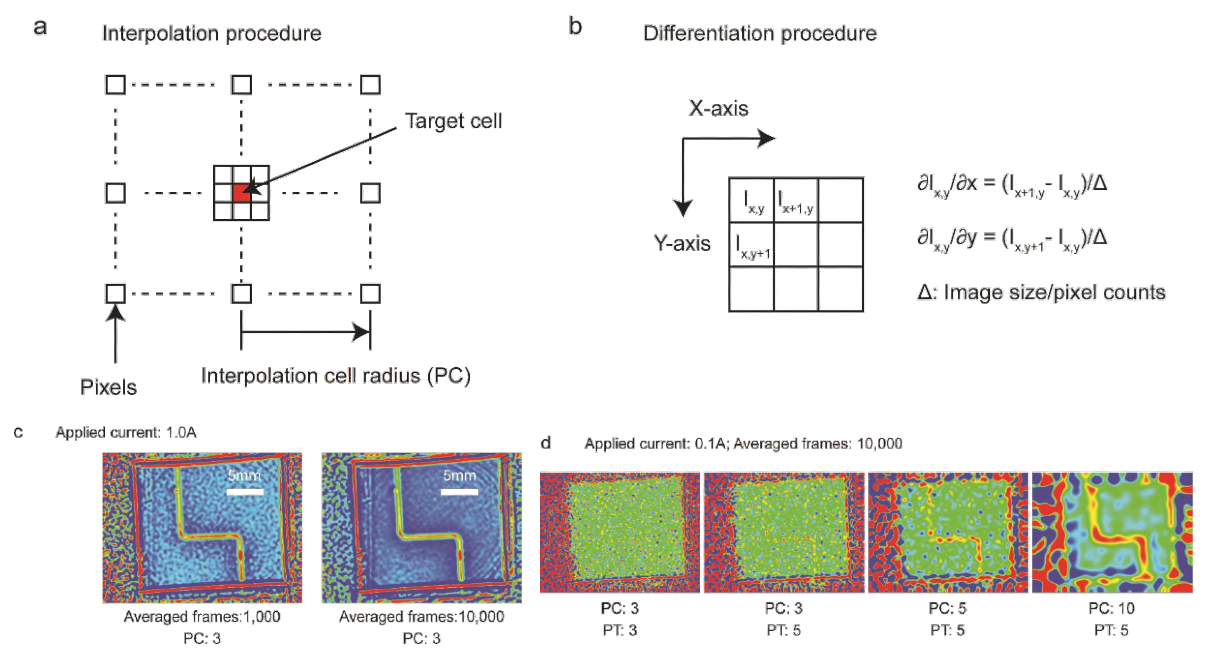
\includegraphics[width=1.0\textwidth]{data/presentation/interp-diff.png}
\end{figure}

\end{frame}

\resetCountingSlides{3}

\begin{frame}
\frametitlecounted{Ալիքատարային անտենայի հետազոտումը}

{\fontsize{9}{9} \selectfont
    ՋԱՕԻՄ֊ի միջոցով հետազոտվել է ալիքատարային անտենայի էլեկտրամագնիսական ճառագայթումը։ Օգտագործվել է Pasternak արտադրության PE9804 WR-90 մոդելի ալիքատարը։
}
\begin{figure}
    \centering
    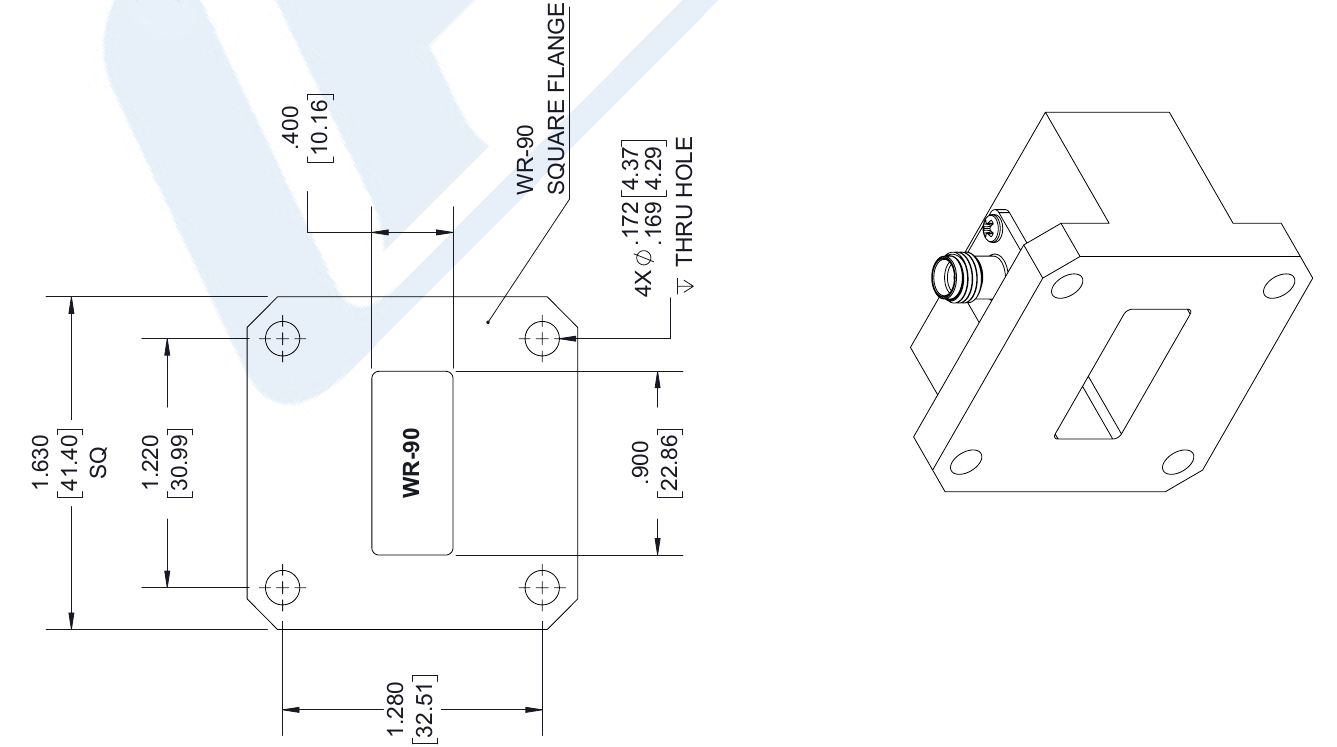
\includegraphics[width=0.9\textwidth]{data/waveguide/waveguide-scheme.png}
\end{figure}

\end{frame}

\begin{frame}
\frametitlecounted{Ալիքատարային անտենայի հետազոտումը}

\begin{tblr}{
  colspec = {X[c,m]X[c,m]},
  rowsep = 6pt,
  hlines = {1pt},
  vlines = {1pt},
}
    Ինդիկատորի թաղանթի նյութը & Ինդիում֊անագի օքսիդ՝ In$_2$O$_3$\cdot SnO$_2$ (Indium-tin oxide - ITO) \\
    Թաղանթի հաստությունը & 100 նմ \\
    Ալիքատարի հեռավորությունը ինդիկատորից & 5 մմ \\
    Ալիքատարի կտրվածքի չափերը & 22.86 մմ\times 10.16 մմ \\
\end{tblr}

\end{frame}

\begin{frame}
\frametitlecounted{Ալիքատարային անտենայի հետազոտումը}

{\fontsize{10}{10} \selectfont Փորձի ընթացքը՝ ամեն մուտքային հզորության համար տրված հաճախային տիրույթում 9 հաճախություններով էլեկտրամագնիսական ալիքների գեներացիայի դեպքում։}

\begin{tblr}{
  colspec = {X[0.5,c,m]X[c,m]},
  rowsep = 6pt,
  hlines = {1pt},
  vlines = {1pt},
}
    Մուտքային հզորությունը & Չափված ալիքների հաճախությունները \\
    0 dBm & [6; 14] ԳՀց, 1 ԳՀց քայլով \\
    3 dBm & [6; 14] ԳՀց, 1 ԳՀց քայլով \\
    6 dBm & [6; 14] ԳՀց, 1 ԳՀց քայլով \\
\end{tblr}

\end{frame}

\resetCountingSlides{4}


\begin{frame}
\frametitlecounted{Փորձի արդյունքները}

\begin{figure}[ht]
    \centering
    \begin{minipage}[c]{0.05\linewidth}
        \rotatebox{90}{0 dBm, 6-14 ԳՀց, մագնիսական դաշտ}
    \end{minipage}
    \hfill
    \begin{minipage}[c]{0.93\linewidth}
    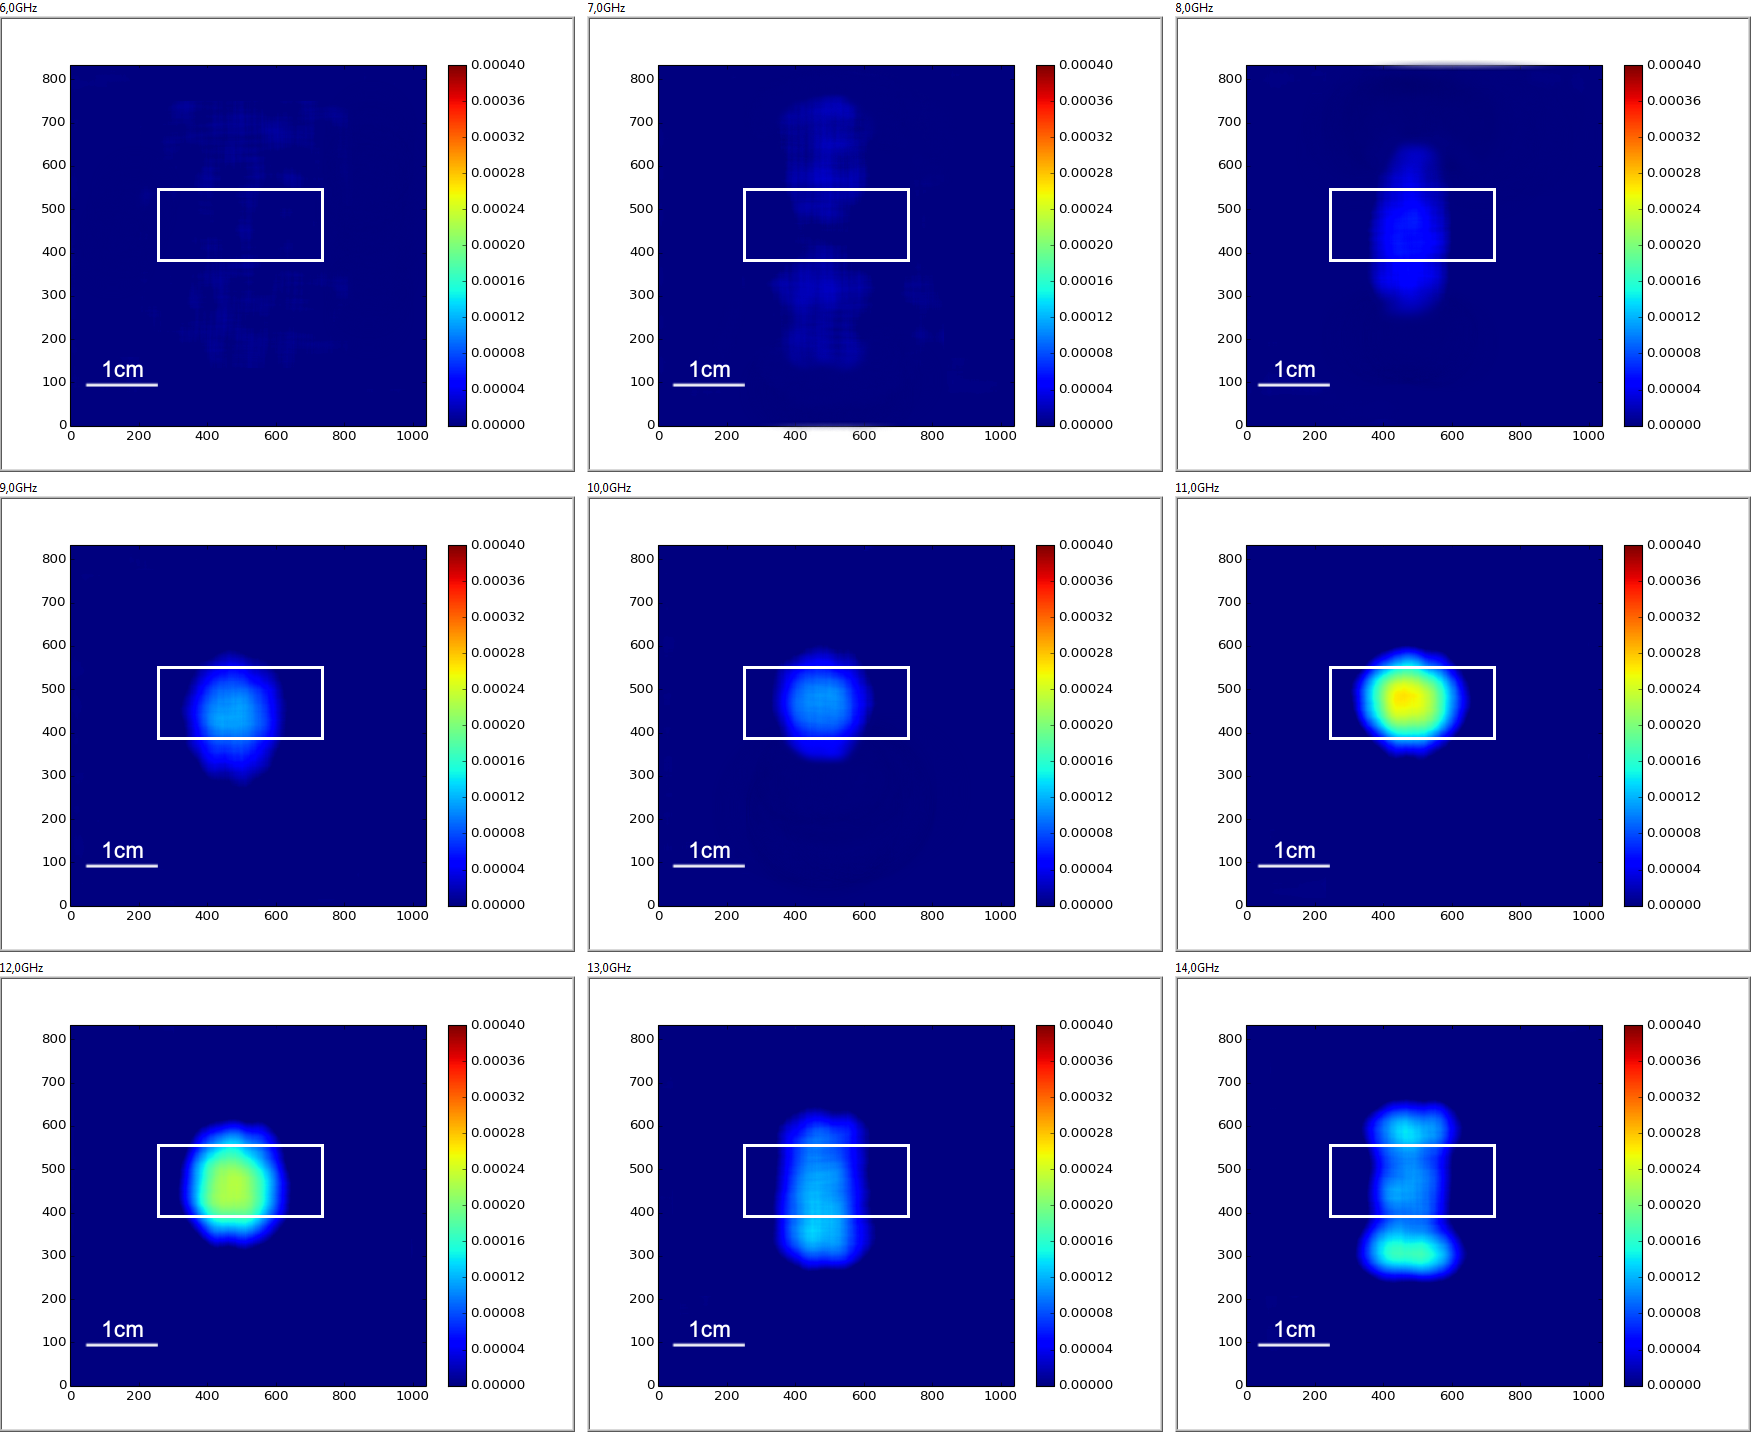
\includegraphics[width=\linewidth]{data/experiment-results/free field of antenna, 6-14ghz, 0dbm generator output, distance 5mm.png}
    \end{minipage}
\end{figure}

\end{frame}


\begin{frame}
\frametitlecounted{Փորձի արդյունքները}

\begin{figure}[ht]
    \centering
    \begin{minipage}[c]{0.05\linewidth}
        \rotatebox{90}{3 dBm, 6-14 ԳՀց, մագնիսական դաշտ}
    \end{minipage}
    \hfill
    \begin{minipage}[c]{0.93\linewidth}
    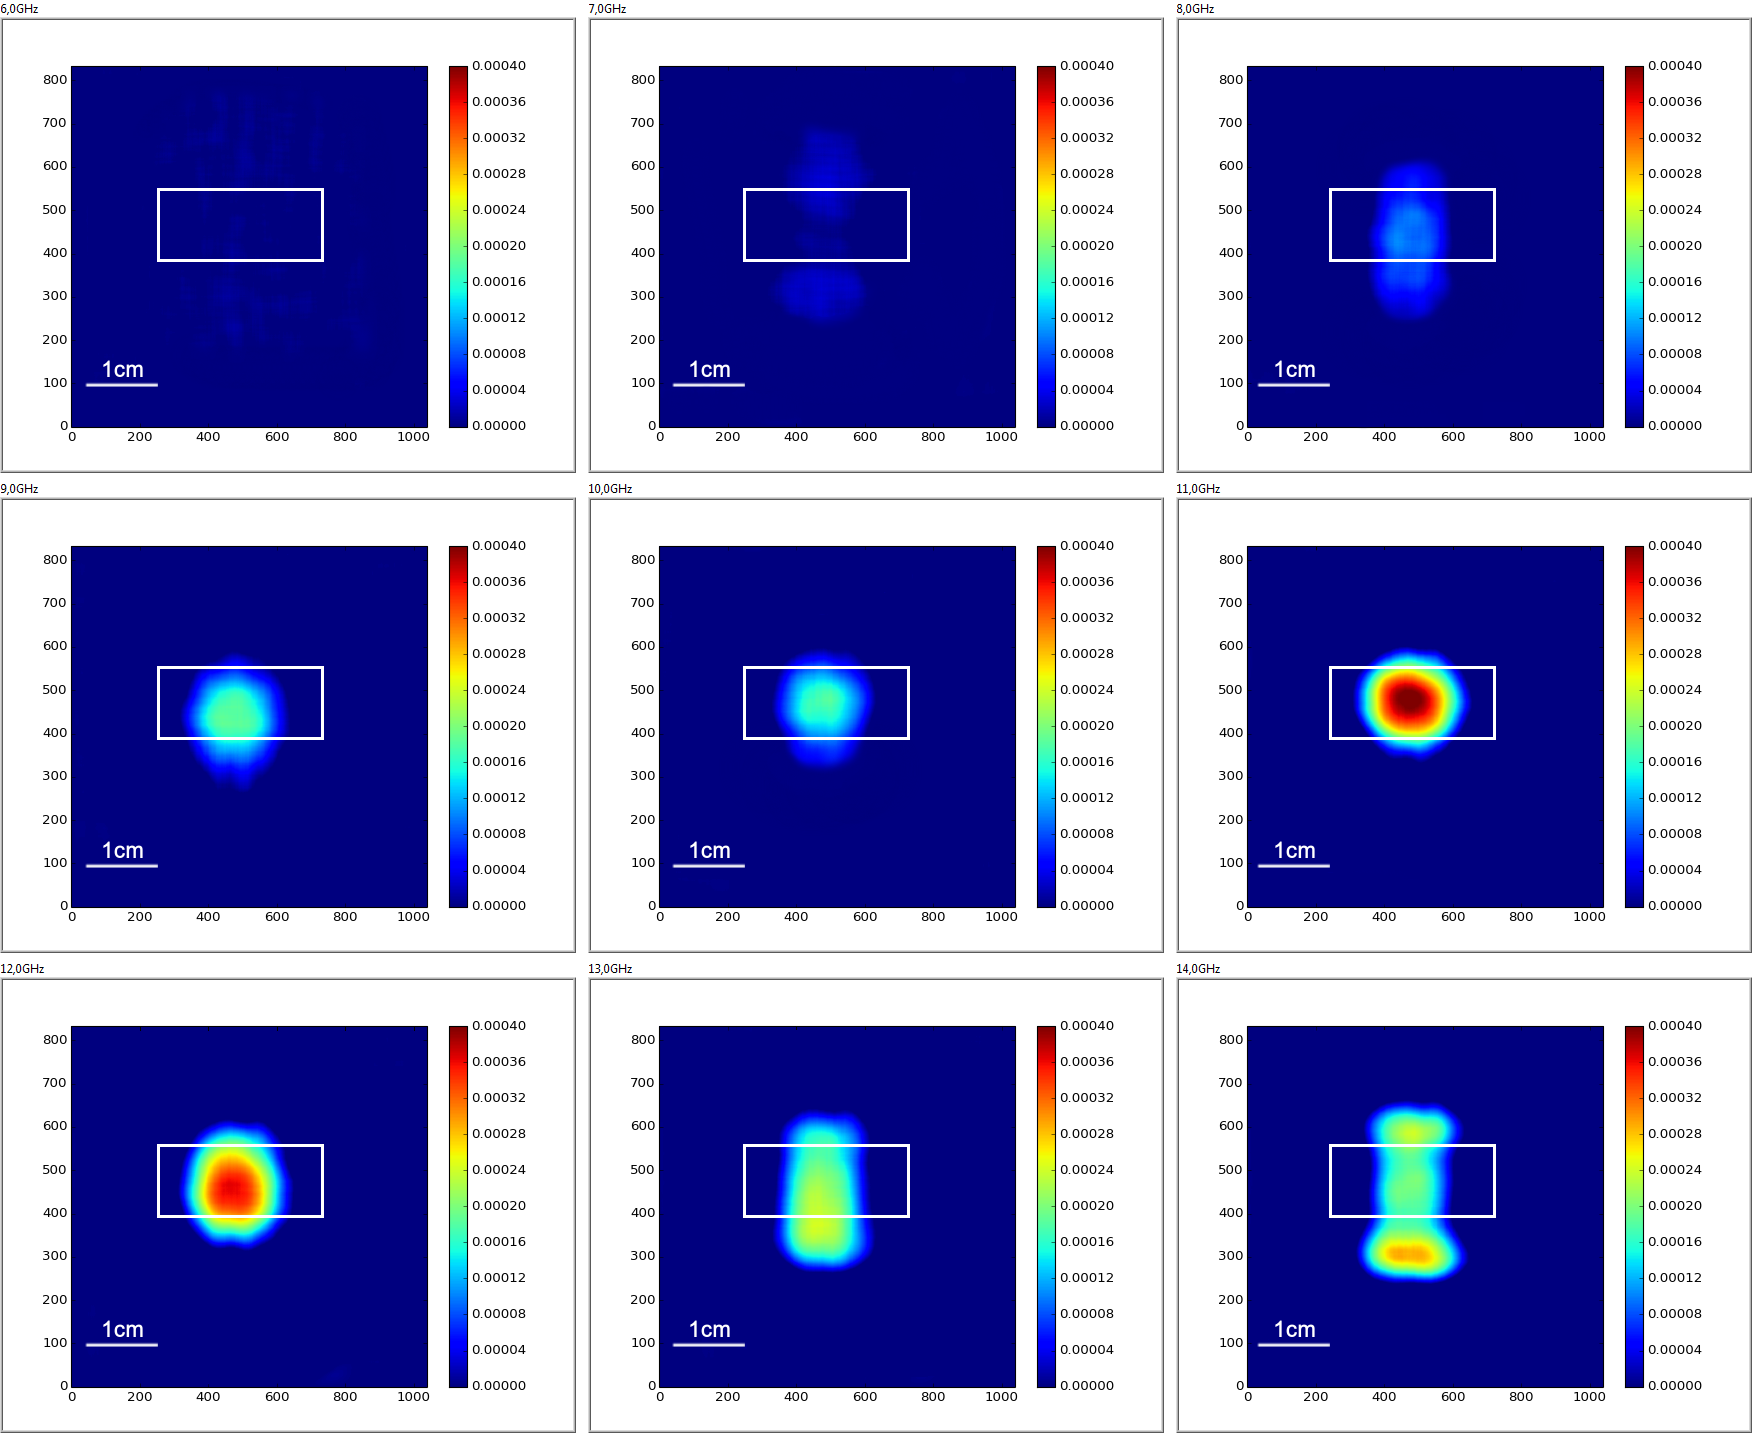
\includegraphics[width=\linewidth]{data/experiment-results/free field of antenna, 6-14ghz, 3dbm generator output, distance 5mm.png}
    \end{minipage}
\end{figure}

\end{frame}


\begin{frame}
\frametitlecounted{Փորձի արդյունքները}

\begin{figure}[ht]
    \centering
    \begin{minipage}[c]{0.05\linewidth}
        \rotatebox{90}{6 dBm, 6-14 ԳՀց, մագնիսական դաշտ}
    \end{minipage}
    \hfill
    \begin{minipage}[c]{0.93\linewidth}
    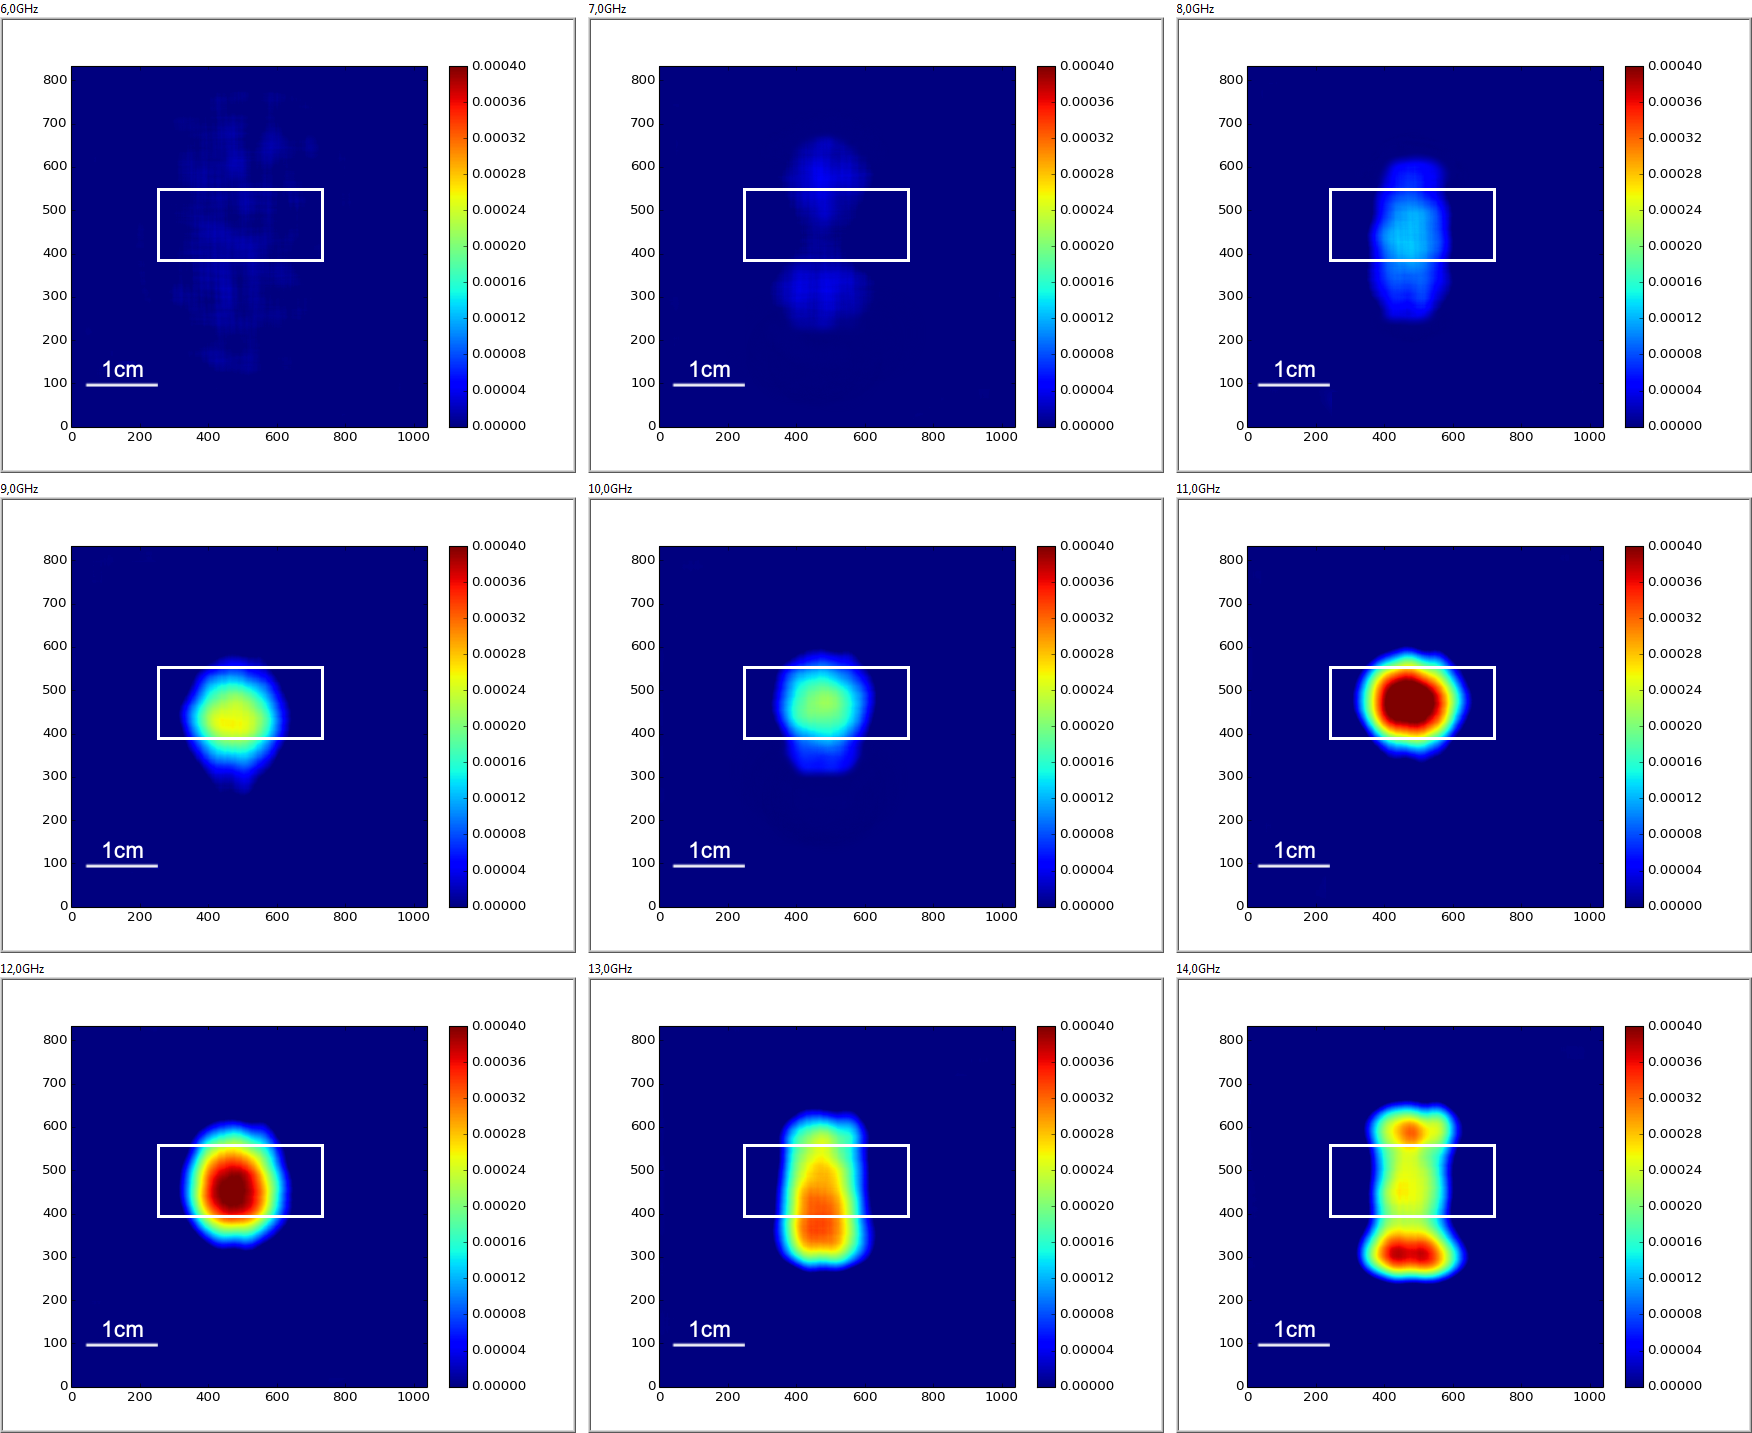
\includegraphics[width=\linewidth]{data/experiment-results/free field of antenna, 6-14ghz, 6dbm generator output, distance 5mm.png}
    \end{minipage}
\end{figure}

\end{frame}

\end{document}
